‘Startside’-fanen for en administrerende bruger er forskellig på nogle punkter, men ellers er layoutet meget det samme. Nyhedsfeedet viser aktiviteter, såsom hvilket barn der påtog sig en pligt, eller at der er blevet anmodet om, at en pligt er færdig, og er klar til at blive evalueret af administrator brugeren. På dette vindue bliver der også vist en notifikation af hvor mange anmodninger, der afventer evaluering. Derudover er der også knapper, som fører brugeren over i et nyt vindue, hvor brugeren kan lave nye pligter eller almindelig bruger profiler, som vil blive lagt op på databasen. Se figur \ref{ForalderUI} for at se dette og de andre faner. Se figur \ref{BarnUI} for statistik fanen, da den er magen til den tilsvarende fane for de almindelige brugere.

Fanen for ‘Pligter’ viser i dette eksempel en samlet liste for alle pligter, hvor ledige pligter bliver vist nederst på listen, påtaget pligter i midten, og pligter, som afventer evaluering af en administrator-bruger, i toppen. I denne faner er der igen en knap til at lave en pligt. Derudover er der en  redigeringsknap, som gør det muligt at ændre på en markeret pligt i listen. Der er også knapper til at acceptere og afvise en pligt, som er anmodet til at være færdige. Hvis anmodningen accepteres, vil den markerede pligt blive opløst i systemet, og en transaktion vil blive sendt til den pågældende bruger. Hvis anmodningen ikke accepteres, vil pligten blive sat tilbage til at være en påtaget pligt. 

'Statistik'-fanen vil her, til forskel fra den almindelige bruger, vise statistik for alle de almindelige brugere i systemet, hvor den almindelige bruger kun ville kunne se statistik for sig selv. Den administrerende brugers liste over saldo ændringer, vil også her indeholde alle de almindelige brugeres overførsler. 

‘Børn’ fanen ville ligesom ‘Pligter’ fanen vise en liste over de almindelige brugere i systemet, og vise diverse informationer angående dem. For eksempel hvilke pligter en bruger har påtaget, samt status på disse pligter og deres saldo. Derudover ville fanen også give muligheder for at lave en ny almindelig bruger til systemet, samt muligheden for at hæve på en af brugernes konti efter anmodning fra brugeren.

\begin{figure}[H]
\centering
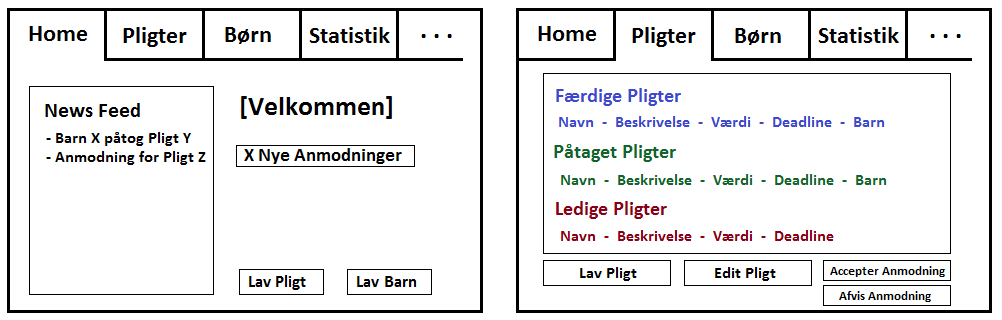
\includegraphics[width=0.9\textwidth]{Billeder/ForalderUI.png}
\caption{Brugergrænseflade illustration for administrerende brugere.}
\label{ForalderUI}
\end{figure}
